% KU Leuven latex presentation template
%
% © 2012 Michael Hofmann
%
% This work is licensed under the Creative Commons Attribution 3.0 Unported License.
% To view a copy of this license, visit
% http://creativecommons.org/licenses/by/3.0/ or send a letter to Creative
% Commons, 444 Castro Street, Suite 900, Mountain View, California, 94041, USA.

\documentclass[t,12pt,dutch
\ifx\beamermode\undefined\else,\beamermode\fi
]{beamer}
%\setbeameroption{show notes}
%\setbeameroption{show only notes}

\usepackage[utf8]{inputenc}
\usepackage[T1]{fontenc}
\usepackage{amsmath}
\usepackage[nohyperlinks]{acronym}
\usepackage{babel,lmodern,graphicx,mathptmx,xspace,wasysym,microtype,booktabs,tabularx,relsize,textcomp,longtable,lipsum,colortbl,eurosym,url,multicol,etoolbox,multimedia,pdfpages,fixltx2e,ifluatex,epstopdf}
\usepackage[olditem,oldenum]{paralist}
\usepackage[babel=true]{csquotes}
\usepackage[thinqspace,amssymb,textstyle]{SIunits}
\usepackage[textsize=tiny]{todonotes}
\usepackage[symbol]{footmisc}
\usepackage[notquote]{hanging}
\usepackage[normalem]{ulem}
\usepackage[mathscr]{euscript}
%\usepackage{lua-visual-debug}

\pdfstringdefDisableCommands{\renewcommand{\sout}{}}
\graphicspath{{figures/}}
% Fix sort order in case the same file exists with multiple extensions
\DeclareGraphicsExtensions{.pdf,.png,.jpeg,.jpg,.eps}
\frenchspacing

\ifluatex\else
% textcomp defines 00B1 wrong, so fix it here
\DeclareUnicodeCharacter{2192}{\ensuremath{\rightarrow}}
\DeclareUnicodeCharacter{2194}{\ensuremath{\leftrightarrow}}
\DeclareUnicodeCharacter{2212}{\ensuremath{-}}
\DeclareUnicodeCharacter{22EE}{\ensuremath{\vdots}}
\DeclareUnicodeCharacter{22EF}{\ensuremath{\cdots}}
\DeclareUnicodeCharacter{00B1}{\ensuremath{\pm}}
\DeclareUnicodeCharacter{00D7}{\ensuremath{\times}}
\DeclareUnicodeCharacter{221E}{\ensuremath{\infty}}
\DeclareUnicodeCharacter{2248}{\ensuremath{\approx}}
\DeclareUnicodeCharacter{2264}{\ensuremath{\leq}}
\DeclareUnicodeCharacter{2265}{\ensuremath{\geq}}
\DeclareUnicodeCharacter{03BC}{\micro}
\DeclareUnicodeCharacter{2206}{\ensuremath{\Delta}}
\fi

\makeatletter
\@ifpackageloaded{xcolor}{%
    \definecolor{kuldefault}{HTML}{00407a}%
    \definecolor{kulbright}{HTML}{52bdec}%
    \definecolor{kulleft}{HTML}{1d8db0}%
    \definecolor{kulright}{HTML}{116e8a}%
    \definecolor{kuldark}{HTML}{123C75}% heading background
    \definecolor{kullight}{HTML}{F0F7FA}% block background
    \definecolor{kulbg}{RGB}{29,141,176}% background fill
    \definecolor{kulyellow}{HTML}{BC8F00}%
    \definecolor{kulorange}{HTML}{BC6E00}%
    \definecolor{kulgreen}{HTML}{007F4F}%
    \definecolor{kulred}{HTML}{FF4422}%
}{}
\makeatother

\newcommand{\m}[1]{\todo[noline,bordercolor=orange!20,backgroundcolor=orange!20]{#1}}

\newcommand{\eg}{e.\,g.\xspace}
\newcommand{\ie}{i.\,e.\xspace}

\addunit{\octave}{octave}
\addunit{\pbdrunit}{\%BDR}
\addunit{\plbdrunit}{\%LBDR}
\addunit{\currentunit}{cu}
\addunit{\pulsespersecondunit}{pps}

\newcommand{\pps}[1]{\unit{#1}{\pulsespersecondunit}}
\newcommand{\hz}[1]{\unit{#1}{\hertz}}
\newcommand{\khz}[1]{\unit{#1}{\kilo\hertz}}
\newcommand{\mhz}[1]{\unit{#1}{\mega\hertz}}
\newcommand{\db}[1]{\unit{#1}{\deci\bel}}
\newcommand{\us}[1]{\unit{#1}{\micro\second}}
\newcommand{\ms}[1]{\unit{#1}{\milli\second}}
\newcommand{\s}[1]{\unit{#1}{\second}}
\newcommand{\pc}[1]{\unit{#1}{\%}}
\newcommand{\pmil}[1]{\unit{#1}{\permil}}
\newcommand{\pcdb}[1]{\unit{#1}{\%\per\deci\bel}}
\newcommand{\de}[1]{\unit{#1}{\degree}}
\newcommand{\uv}[1]{\unit{#1}{\micro\volt}}
\newcommand{\nv}[1]{\unit{#1}{\nano\volt}}
\newcommand{\bdr}[1]{\unit{#1}{\pbdrunit}}
\newcommand{\lbdr}[1]{\unit{#1}{\plbdrunit}}
\newcommand{\cu}[1]{\unit{#1}{\currentunit}}
\newcommand{\nhl}[1]{\unit{#1}{\deci\bel{}\textnormal{nHL}}}
\newcommand{\hl}[1]{\unit{#1}{\deci\bel{}\textnormal{HL}}}
\newcommand{\spl}[1]{\unit{#1}{\deci\bel{}\textnormal{SPL}}}
\newcommand{\spla}[1]{\unit{#1}{\deci\bel{}\textnormal{SPL(A)}}}
\newcommand{\dbfs}[1]{\unit{#1}{\deci\bel{}\textnormal{FS}}}
\newcommand{\pespl}[1]{\unit{#1}{\deci\bel{}\textnormal{peSPL}}}
\newcommand{\pespla}[1]{\unit{#1}{\deci\bel{}\textnormal{peSPL(A)}}}
\newcommand{\sd}[1]{\ensuremath{\textnormal{SD}=#1}}
\newcommand{\se}[1]{\ensuremath{\textnormal{SE}=#1}}
\newcommand{\ir}[1]{\ensuremath{\textnormal{IR}=#1}}
\newcommand{\el}[2]{\ensuremath{\textnormal{#1}_{\textnormal{#2}}}}

% pandoc >=1.14
\providecommand{\tightlist}{\setlength{\itemsep}{0pt}\setlength{\parskip}{0pt}}

\newcommand{\deflen}[2]{%
    \expandafter\newlength\csname #1\endcsname
    \expandafter\setlength\csname #1\endcsname{#2}%
}




%% From pandoc default template
%% End pandoc

\mode<presentation>

%\hypersetup{pdfpagemode=FullScreen}

\setbeamercolor{structure}{fg=kulbright}
\setbeamercolor{title}{fg=white}
\setbeamercolor{footline}{parent=title}
\setbeamercolor{normal text}{fg=kuldefault}
\setbeamercolor{item}{parent=normal text}
\setbeamercolor{section in toc}{parent=normal text}
\setbeamercolor{footline extra}{fg=white}
\setbeamerfont{title}{size=\Large}
\setbeamerfont{tiny structure}{series=\bfseries}
\setbeamerfont{caption}{}

\setbeamersize{text margin left=0.8cm}
\setbeamersize{text margin right=0.8cm}
\setbeamersize{sidebar width left=0cm}

\setbeamertemplate{navigation symbols}{}
\setbeamertemplate{itemize item}{\footnotesize\raise1pt\hbox{\textbullet}}
\setbeamertemplate{itemize subitem}{--}
\setbeamertemplate{itemize subsubitem}{\tiny\raise1.5pt\hbox{\textbullet}}

\setlength\leftmargini{1em}
\setlength\leftmarginii{1em}
\setlength\leftmarginiii{1em}

\defbeamertemplate{background canvas}{title}
{%
    \pgfdeclarehorizontalshading{bgshading}{8.70cm}{color(0cm)=(kulleft); color(\the\paperwidth)=(kulright)}%
    \vbox to 8.70cm{%
        \pgfuseshading{bgshading}\hspace*{-1.6cm}%
    }%
    \hskip-\paperwidth%
    \hskip1.6cm%
    \vbox to \paperheight{%
        \vskip0.5cm\hskip0.5cm
\includegraphics[width=2.83cm]{templates/kuleuven}%
        \vskip0.99cm\hskip0.76cm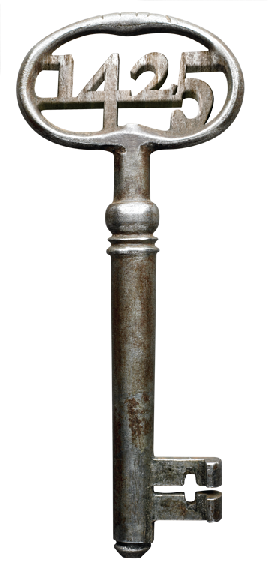
\includegraphics[width=2.84cm]{templates/key}%
        \vskip-0.57cm\hskip11.61cm\includegraphics[width=0.58cm]{templates/sedes}\hspace*{-1cm}%
        \vfill
    }%
}

\defbeamertemplate{background canvas}{grid}
{%
    \begin{tikzpicture}[remember picture,overlay,every node/.style={anchor=center}]
        \foreach \d in {0,...,20} {
            \draw[gray] (\d,0) -- (\d,-20);
            \draw[gray] (0,-\d) -- (20,-\d);
            \draw[lightgray] (\d+0.5,0) -- (\d+0.5,-20);
            \draw[lightgray] (0,-\d-0.5) -- (20,-\d-0.5);
            \node[anchor=north,red,font=\tiny] at (\d,0) {\d};
            \node[anchor=west,red,font=\tiny] at (0,-\d) {\d};
        }
    \end{tikzpicture}
}



% add a macro that saves its argument
\newcommand{\footlineextra}[1]{\gdef\insertfootlineextra{#1}}
\newbox\footlineextrabox


% add a beamer template that sets the saved argument in a box.
% The * means that the beamer font and color "footline extra" are automatically added.
\defbeamertemplate*{footline extra}{default}{
    %\begin{beamercolorbox}[ht=2.25ex,dp=1ex,leftskip=\Gm@lmargin]{footline extra}
    \begin{beamercolorbox}[ht=0.37cm,dp=0.25cm,wd=0.4\paperwidth,left,leftskip=2ex]{footline extra}
    \insertfootlineextra
    %\par\vspace{2.5pt}
    \end{beamercolorbox}
}

\defbeamertemplate{background canvas}{plain}{}

\defbeamertemplate{footline}{large}
{%
    \pgfdeclarehorizontalshading{bgshading}{0.62cm}{color(0cm)=(kulleft); color(\the\paperwidth)=(kulright)}%
    \vskip.3cm% make room for the logo
    \parbox[t][0.62cm]{\paperwidth}{\pgfuseshading{bgshading}}\par%
    \vskip-0.62cm%
    \begin{beamercolorbox}[ht=0.37cm,dp=0.25cm,center]{page number in head/foot}%
    \insertframenumber%
    \end{beamercolorbox}%
    \vskip-0.92cm%
    \parbox[t][0.92cm]{\paperwidth}{\hskip10.33cm
\includegraphics[width=2.10cm]{templates/kuleuven}}\par%

    % set the box with the extra footline material but make it add no vertical space
    \setbox\footlineextrabox=\vbox{\usebeamertemplate*{footline extra}}
    \vskip -\ht\footlineextrabox
    \vskip -\dp\footlineextrabox
    \box\footlineextrabox%
}

% patch \begin{frame} to reset the footline extra material
\makeatletter
\let\beamer@original@frame=\frame
\def\frame{\gdef\insertfootlineextra{}\beamer@original@frame}
\footlineextra{}
\makeatother


\defbeamertemplate{footline}{nopagenumber}
{%
    \pgfdeclarehorizontalshading{bgshading}{0.62cm}{color(0cm)=(kulleft); color(\the\paperwidth)=(kulright)}%
    \vskip.3cm% make room for the logo
    \parbox[t][0.62cm]{\paperwidth}{\pgfuseshading{bgshading}}\par%
    \vskip-0.62cm%
    \begin{beamercolorbox}[ht=0.37cm,dp=0.25cm,center,ignorebg]{page number in head/foot}%
    %
    \end{beamercolorbox}%
    \vskip-0.92cm%
    \parbox[t][0.92cm]{\paperwidth}{\hskip10.33cm
\includegraphics[width=2.10cm]{templates/kuleuven}}\par%
}

\defbeamertemplate{footline}{small}
{%
    \vskip.3cm% make room for the logo
    \begin{beamercolorbox}[ht=0.37cm,dp=0.25cm,center,ignorebg]{normal text}%
    \mdseries\insertframenumber%
    \end{beamercolorbox}%
}

\setbeamertemplate{footline}[large]

\setbeamertemplate{frametitle}
{%
    \nointerlineskip%
    \vskip.28cm%
    {\usebeamercolor[fg]{framesubtitle}\usebeamerfont{framesubtitle}\insertsupertitle\strut\par}%
    \vskip-.2cm%
    {\usebeamercolor[fg]{frametitle}\usebeamerfont{frametitle}\insertframetitle\strut\par}%
    \vskip-.3cm%
}

\setbeamertemplate{title page}
{
    \vbox{}%
    \vskip2.8cm%
    \vbox to 6.5cm{%
        \hskip2.8cm%
        \begin{minipage}{7.9cm}
            \begin{beamercolorbox}{title}
                \usebeamerfont{title}%
                \inserttitle\par%
                \ifx\insertsubtitle\undefined%
                \else%
                    \vskip0.25em%
                    {\usebeamerfont{subtitle}\usebeamercolor[fg]{subtitle}\insertsubtitle\par}%
                \fi%
            \end{beamercolorbox}%
            \vskip1em\par
            \begin{beamercolorbox}{author}
                \usebeamerfont{author}\usebeamercolor[fg]{subtitle}%
                \insertauthor
            \end{beamercolorbox}
            \begin{beamercolorbox}{institute}
                \usebeamerfont{institute}\usebeamercolor[fg]{subtitle}%
                \insertinstitute
                \end{beamercolorbox}
            \begin{beamercolorbox}{date}
                \usebeamerfont{date}\usebeamercolor[fg]{subtitle}%
                \insertdate
            \end{beamercolorbox}%
        \end{minipage}%
        \vfill
    }
}

\mode<all>

\newcommand{\inlinesound}[2]{\movie[inlinesound,encoding=Signed,samplingrate=44100]{#1}{#2}}

% disable for now as otherwise all commands that go between frames generated by
% the filter will result in duplicate toc lines
\renewcommand{\addcontentsline}[3]{}

\newcommand{\largefooter}{\setbeamertemplate{footline}[large]}
\newcommand{\emptyfooter}{\setbeamertemplate{footline}[nopagenumber]}
\newcommand{\smallfooter}{\setbeamertemplate{footline}[small]}
\newcommand{\nofooter}{\setbeamertemplate{footline}[nofooter]}

\newcommand{\sectiontoc}{\AtBeginSection[]{{
    \nosupertitle
    \emptyfooter
    \begin{frame}[noframenumbering]{Outline}
                \tableofcontents[currentsection]
            \end{frame}
    \largefooter
}}}

\newcommand{\subsectiontoc}{\AtBeginSubsection[]{{
    \nosupertitle
    \emptyfooter
    \begin{frame}[noframenumbering]{Outline}
                \tableofcontents[currentsection,currentsubsection]
           \end{frame}
    \largefooter
}}}

\newcommand{\notoc}{\AtBeginSection[]{}\AtBeginSubsection[]{}}

\newcommand{\nosupertitle}{\renewcommand{\insertsupertitle}{}}
\newcommand{\sectiontitle}{\renewcommand{\insertsupertitle}{\insertsectionhead}}
\newcommand{\subsectiontitle}{\renewcommand{\insertsupertitle}{\insertsectionhead\ifx\insertsubsectionhead\empty\else{} -- \insertsubsectionhead\fi}}

% animations do not work atm as figures are set on independent frames
\newcommand{\slidefig}[2]{\usebackgroundtemplate{\parbox[c][\paperheight][c]{\paperwidth}{\centering\includegraphics#1[height=\paperheight,width=\paperwidth,keepaspectratio]{#2}}}\begin{frame}[plain]\end{frame}\usedefaultcanvas}

\newcommand{\usedefaultcanvas}{\setbeamertemplate{background canvas}[\defaultcanvas]}
\newcommand{\gridcanvas}{\renewcommand{\defaultcanvas}{grid}\usedefaultcanvas}
\newcommand{\plaincanvas}{\renewcommand{\defaultcanvas}{plain}\usedefaultcanvas}

\newcommand{\insertsupertitle}{}






\newcommand{\defaultcanvas}{plain}


% Defining a new coordinate system for the page:
%
% ----------------
% |(0,1)    (1,1)|
% |              |
% |(0,0)    (1,0)|
% ----------------
\makeatletter
\def\parsecomma#1,#2\endparsecomma{\def\page@x{#1}\def\page@y{#2}}
\tikzdeclarecoordinatesystem{page}{
    \parsecomma#1\endparsecomma
    \pgfpointanchor{current page}{north east}
    % Save the upper right corner
    \pgf@xc=\pgf@x%
    \pgf@yc=\pgf@y%
    % save the lower left corner
    \pgfpointanchor{current page}{south west}
    \pgf@xb=\pgf@x%
    \pgf@yb=\pgf@y%
    % Transform to the correct placement
    \pgfmathparse{(\pgf@xc-\pgf@xb)*\page@x+(\pgf@xb)}
    \expandafter\pgf@x\expandafter=\pgfmathresult pt
    \pgfmathparse{(\pgf@yc-\pgf@yb)*\page@y+(\pgf@yb)}
    \expandafter\pgf@y\expandafter=\pgfmathresult pt
}
\makeatother

% Example:
%\begin{tikzpicture}[remember picture,overlay,every node/.style={anchor=center}]
%  \node at (page cs:0.5,0.3) {0.5,0.3};
%  \node at (page cs:0,0) {0,0};
%  \draw(page cs:0,0) -- (page cs:1,1);
%  \draw[thick,red] (page cs:0,0) rectangle (page cs:1,1);
%  \draw[thick,green] (page cs:0.2,0.2) rectangle (page cs:0.8,0.8);
%\end{tikzpicture}

\setcounter{secnumdepth}{0}

\title{Hyperspectrale afbeeldingscompressie via tensordecomposities}
\author{\mbox{Wouter Baert} \and \mbox{Promotor: dr. prof. ir. Karl Meerbergen} \and \mbox{Co-promotor: dr. Nick Vannieuwenhoven}}
\date{28 juni 2019}
\institute{}

% Own header
\setbeamertemplate{bibliography item}{\insertbiblabel}
\usepackage[]{algorithm2e}
\usepackage{subcaption}
\usepackage{graphicx,array}

\newcolumntype{C}[1]{>{\centering\let\newline\\\arraybackslash\hspace{0pt}}m{#1}}
\newcolumntype{L}[1]{>{\raggedright\let\newline\\\arraybackslash\hspace{0pt}}m{#1}}

\begin{document}

\setbeamertemplate{background canvas}[title]

\begin{frame}[plain,noframenumbering]
    \titlepage
\end{frame}

\usedefaultcanvas


%\emptyfooter
%\begin{frame}[noframenumbering]{Outline}
%        \tableofcontents
%    \end{frame}
%\largefooter

%\section{First Section}\label{first-section}

% Inleiding

\begin{frame}{Hyperspectrale afbeeldingen}

\begin{figure}[H]
\centering
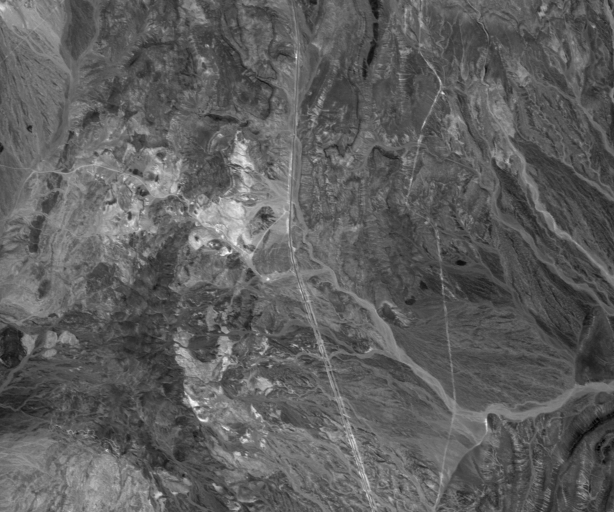
\includegraphics[scale=0.3]{images/cuprite_bands_0-32.png}
\caption{Cuprite, Nevada (VS): banden 0-31 (bron: AVIRIS \cite{ref:ehu_aviris_cuprite})}
\end{figure}

\end{frame}

\begin{frame}{Hyperspectrale afbeeldingen}

\begin{figure}[H]
\centering
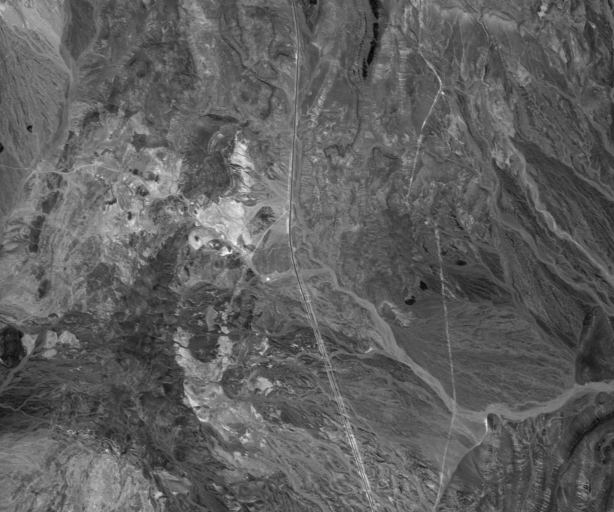
\includegraphics[scale=0.3]{images/cuprite_bands_32-63.png}
\caption{Cuprite, Nevada (VS): banden 32-62 (bron: AVIRIS \cite{ref:ehu_aviris_cuprite})}
\end{figure}

\end{frame}

\begin{frame}{Hyperspectrale afbeeldingen}

\begin{figure}[H]
\centering
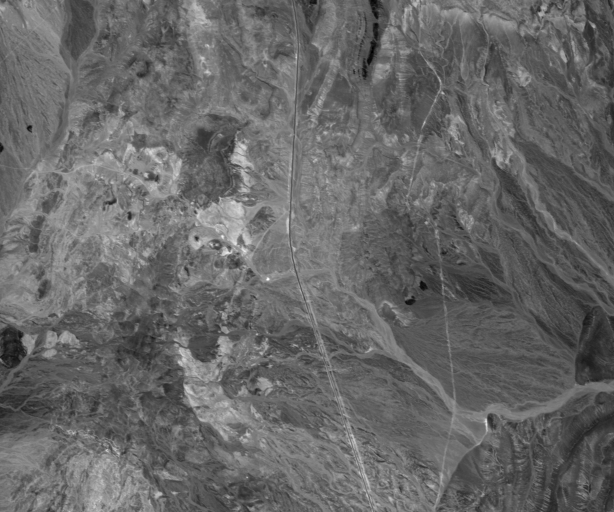
\includegraphics[scale=0.3]{images/cuprite_bands_63-95.png}
\caption{Cuprite, Nevada (VS): banden 63-94 (bron: AVIRIS \cite{ref:ehu_aviris_cuprite})}
\end{figure}

\end{frame}

\begin{frame}{Hyperspectrale afbeeldingen}

\begin{figure}[H]
\centering
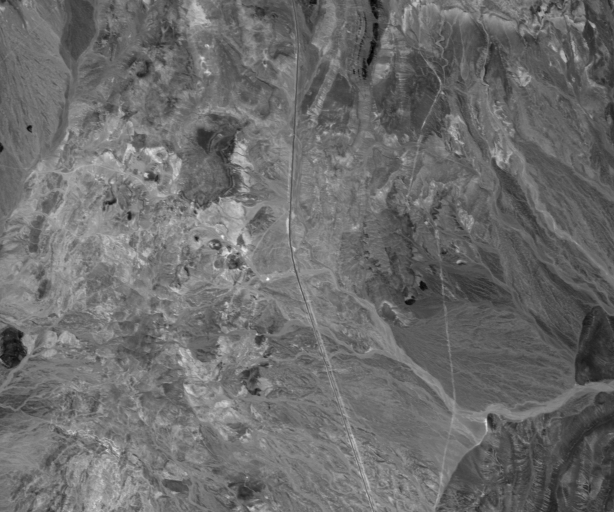
\includegraphics[scale=0.3]{images/cuprite_bands_95-127.png}
\caption{Cuprite, Nevada (VS): banden 95-126 (bron: AVIRIS \cite{ref:ehu_aviris_cuprite})}
\end{figure}

\end{frame}

\begin{frame}{Hyperspectrale afbeeldingen}

\begin{figure}[H]
\centering
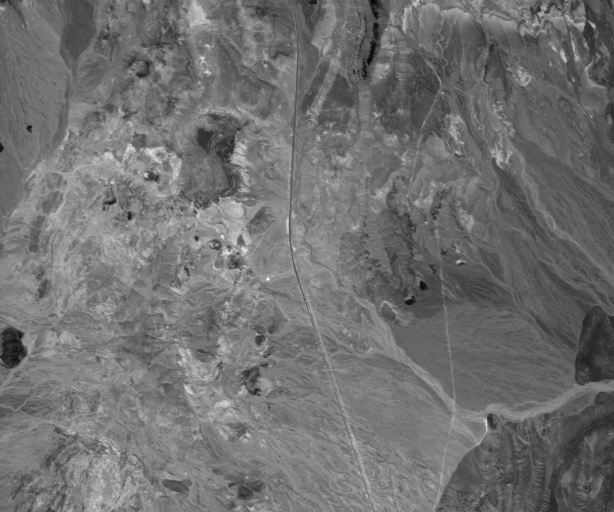
\includegraphics[scale=0.3]{images/cuprite_bands_127-158.png}
\caption{Cuprite, Nevada (VS): banden 127-157 (bron: AVIRIS \cite{ref:ehu_aviris_cuprite})}
\end{figure}

\end{frame}

\begin{frame}{Hyperspectrale afbeeldingen}

\begin{figure}[H]
\centering
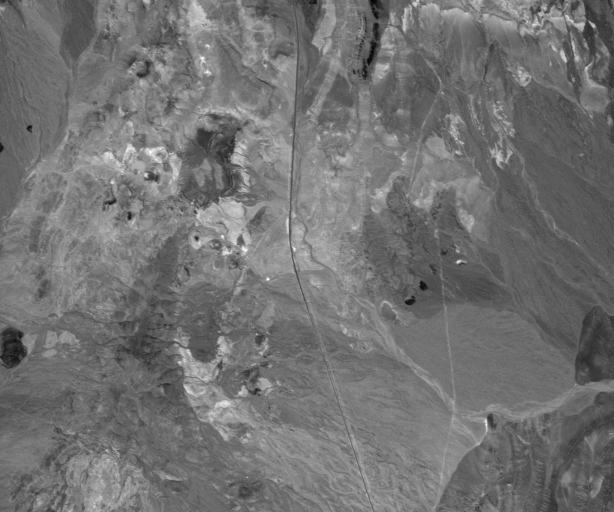
\includegraphics[scale=0.3]{images/cuprite_bands_158-190.png}
\caption{Cuprite, Nevada (VS): banden 158-189 (bron: AVIRIS \cite{ref:ehu_aviris_cuprite})}
\end{figure}

\end{frame}

% Achtergrond

\begin{frame}{}
\begin{center}
\topskip0pt
\vspace*{\fill}
\vspace*{\fill}
\Huge
Achtergrond
\normalsize
\vspace*{\fill}
\end{center}
\end{frame}

\begin{frame}{Algemeen}

\begin{itemize}
\item Compressiefactor = $\frac{\text{originele grootte}}{\text{gecomprimeerde grootte}}$
\item Compressiefout = $\frac{||\text{gecomprimeerde data } - \text{ originele data}||_F}{||\text{originele data}||_F}$
\end{itemize}

\end{frame}

\begin{frame}{Singulierewaardenontbinding (SVD)}

$A = U \Sigma V^T$ met 
\begin{itemize}
\item $A \in \mathbb{R}^{m \times n}$, $U \in \mathbb{R}^{m \times m}$, $\Sigma \in \mathbb{R}^{m \times n}$ en $V \in \mathbb{R}^{n \times n}$
\item $U$ en $V$ orthogonaal
\item $\Sigma$ diagonaal en positief, van groot naar klein
\newline
\end{itemize}
$A \approx \widetilde{U} \widetilde{\Sigma} \widetilde{V}^T$ met 
\begin{itemize}
\item $A \in \mathbb{R}^{m \times n}$, $\widetilde{U} \in \mathbb{R}^{m \times k}$, $\widetilde{\Sigma} \in \mathbb{R}^{k \times k}$ en $\widetilde{V} \in \mathbb{R}^{n \times k}$
\item $\widetilde{U}$, $\widetilde{V}$ eerste $k$ kolommen $U, V$
\item $\widetilde{\Sigma}$ eerste $k$ diagonaalelementen $\Sigma$
\item Beste rang-$k$ benadering van $A$ (Frobeniusnorm)
\end{itemize}

\end{frame}

\begin{frame}{Tensoren en $n$-mode product (Kolda, Bader \cite{ref:kolda})}

\begin{itemize}
\item $A$ is tensor met $d$ modes
\item $A \times_k U$ met $U \in \mathbb{R}^{r_k \times n_k}$ betekent:
\begin{enumerate}
\item Neem mode-$k$-vezels (lengte $n_k$)
\item Transformeer elke vector $a$ naar $Ua$ (lengte $r_k$)
\item Vouw terug in tensor
\end{enumerate}
\end{itemize}

\begin{figure}[H]
\centering
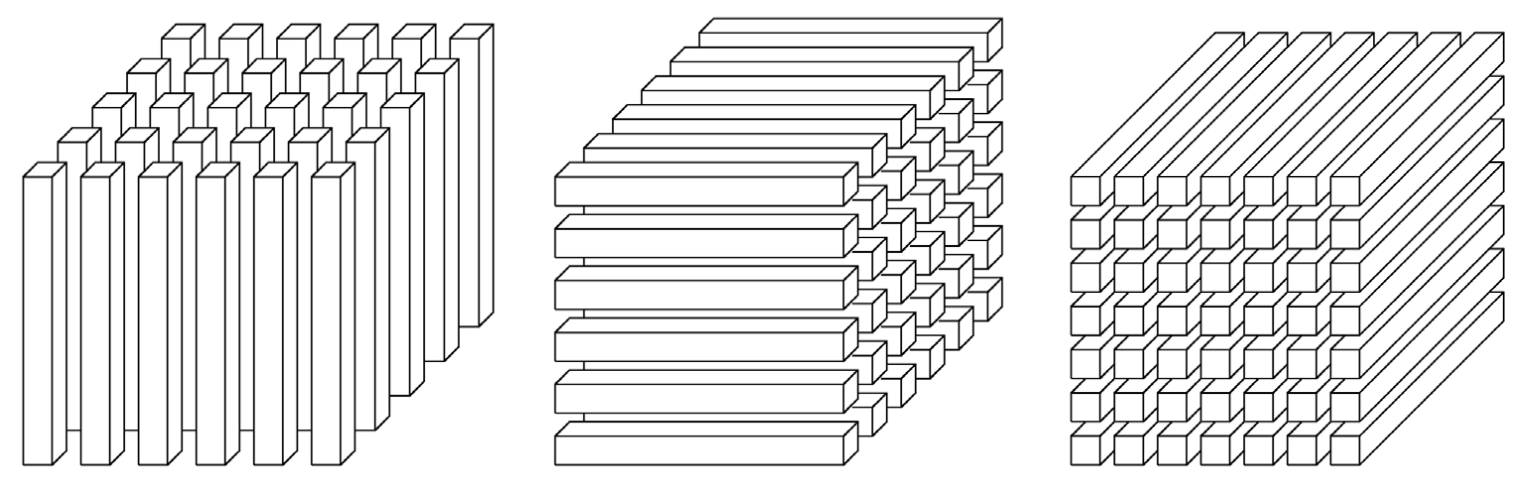
\includegraphics[scale=0.13]{images/fibers.png}
\caption{Vezels van een 3D-tensor (bron: Kolda, Bader \cite{ref:kolda})}
\end{figure}

\end{frame}

\begin{frame}{Tucker-decompositie (Tucker \cite{ref:tucker})}

\begin{itemize}
\item Stel $A$ voor als kerntensor $B$ en factormatrices $U_1, \dots, U_d$ zodat\\
$A \approx B \times_1 U_1 \dots \times_d U_d$\\
met $A \in \mathbb{R}^{n_1 \times n_2 \times \dots \times n_d}$, $B \in \mathbb{R}^{r_1 \times r_2 \times \dots \times r_d}$, $U_i \in \mathbb{R}^{n_i \times r_i}$
\item Factormatrices kunnen op verschillende manieren gekozen worden
\end{itemize}

\end{frame}

\begin{frame}{ST-HOSVD (Vannieuwenhoven, Vandebril, Meerbergen \cite{ref:st_hosvd})}

\begin{figure}[H]
\centering
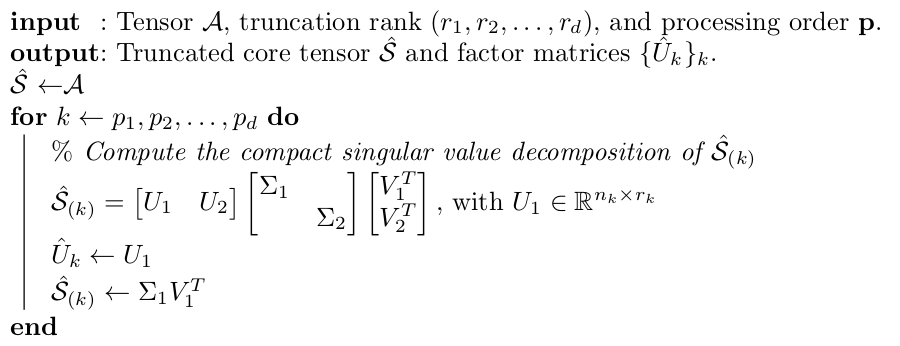
\includegraphics[scale=0.35]{images/ST-HOSVD.png}
\caption{ST-HOSVD-algoritme (bron: VVM \cite{ref:st_hosvd})}
\end{figure}

\end{frame}

% Eigen onderzoek

\begin{frame}{}
\begin{center}
\topskip0pt
\vspace*{\fill}
\vspace*{\fill}
\Huge
Eigen onderzoek
\normalsize
\vspace*{\fill}
\end{center}
\end{frame}

% Tucker-gebaseerde compressie

\begin{frame}{}
\begin{center}
\topskip0pt
\vspace*{\fill}
\vspace*{\fill}
\Huge
Tucker-gebaseerde compressie
\normalsize
\vspace*{\fill}
\end{center}
\end{frame}

\begin{frame}{Overzicht}
\begin{enumerate}
\item ST-HOSVD-compressie
\item Orthogonaliteitscompressie
\item Quantisatie
\item Encodering
\end{enumerate}
\end{frame}

\begin{frame}{Versnellen ST-HOSVD}

\begin{itemize}

\item Modevolgorde: eerst spectrale mode, best comprimeerbaar

\item Methode met Gram-matrix i.p.v. SVD:
\begin{itemize}

\item SVD van $A \in \mathbb{R}^{m \times n}$ met $m < n$: $O(m^2 n)$

\item Eigenwaardenontbinding van $A A^T$:
\begin{itemize}
\item Berekenen $A A^T$: $O(m^2 n)$
\item Berekenen eigenwaardenontbinding: $O(m^3)$
\end{itemize}

\item Voorbeeld:
\begin{table}[H]
\centering
\begin{tabular}{|l|l|l|}
\hline
Methode & Relatieve fout & Compressietijd (s)\\ \hline
\input{data/gram-matrix.tex}
\end{tabular}
\end{table}

\end{itemize}
\end{itemize}
\end{frame}

\begin{frame}{Orthogonaliteitscompressie}

\begin{itemize}
\item Voorbeelden ruimte-inname factormatrices:
\begin{itemize}
\item Cuprite: 64\%
\item Mauna Kea: 55\%
\end{itemize}
\item Maar: $r (r - 1)/2$ orthogonaliteitsconstraints ($r$ kolommen)!
\end{itemize}

\end{frame}

\iffalse

\begin{frame}{Orthogonaliteitscompressie: stelsels}

\begin{center}
$
\begin{bmatrix}
A & b & \dots \\[0.3em]
C & x & \dots \\[0.3em]
\end{bmatrix}
$
met $A \in \mathbb{R}^{(n-k) \times k}, C \in \mathbb{R}^{k \times k}, b \in \mathbb{R}^{n - k}, x \in \mathbb{R}^{k}$
\end{center}

\begin{itemize}
\item Orthogonaliteit: $\Rightarrow C^T x = -A^T b$
\item Volledige driehoek herberekenen:
\begin{itemize}
\item Fouten stapelen op, erg grote eindfout
\item Grote decompressietijd: $O(r^4)$
\end{itemize}
\end{itemize}

\begin{figure}[H]
\centering
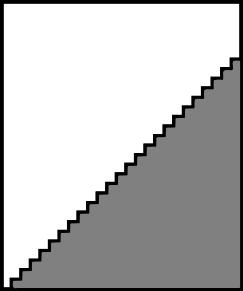
\includegraphics[scale=0.8]{images/orthogonality_compression1.png}
\end{figure}

\end{frame}

\fi

\begin{frame}{Orthogonaliteitscompressie: Householder-reflecties}
\[
H_i = I - 2 v_i v_i^T
\]
\[
U = H_1 H_2 \dots H_r \quad \text{met dimensie } v_i = n + 1 - i
\]
\begin{itemize}
\item Fout: erg klein, numeriek OK want weggelaten waarden zijn specifiek gekozen
\item Compressiefactor: perfect, $r (r - 1)/2$ minder opgeslagen waarden
\item (De)compressietijd: geen probleem, $O(r^3)$
\end{itemize}
\end{frame}

\begin{frame}{Quantisatie}
\begin{itemize}
\item Floating-point getallen $\rightarrow$ kleine discrete verzameling
\item ``Quantiseren $x_1, \dots, x_n$ naar $b$ bits'':\\
$x_i \rightarrow round(\frac{2^b - 1}{max(x_1, \dots, x_n) - min(x_1, \dots, x_n)} (x_i - min(x_1, \dots, x_n)))$
\end{itemize}
\end{frame}

\begin{frame}{Quantisatie: kerntensor}

\begin{itemize}
\item ST-HOSVD concentreert energie in lage indices
\item Definitie laag (schil):
\end{itemize}

\begin{figure}[H]
\centering
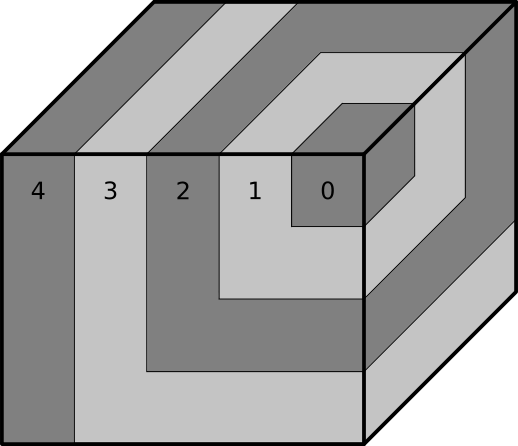
\includegraphics[scale=0.6]{images/core_tensor_layers.png}
\end{figure}

\end{frame}

\begin{frame}{Quantisatie: kerntensor}

\begin{figure}[H]
\centering
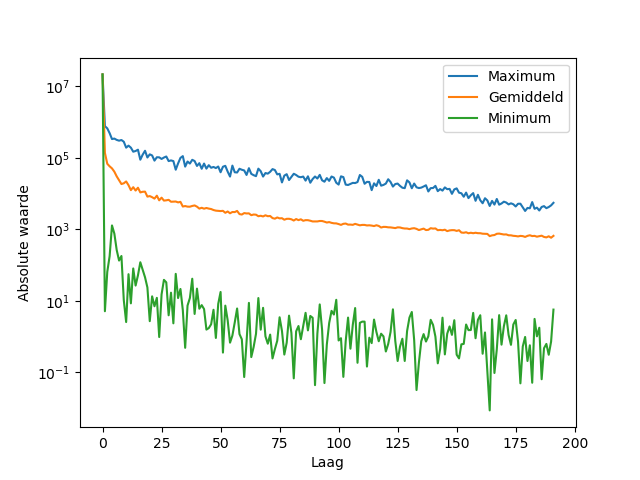
\includegraphics[scale=0.5]{images/core_tensor_values_distribution.png}
\end{figure}

\end{frame}

\begin{frame}{Quantisatie: kerntensor}
\begin{itemize}
\item Factormatrices genormaliseerd $\rightarrow$ absolute fout op elke positie kerntensor even significant
\item Gevolg: eerste lagen ongequantiseerd opslaan
\item Verschillende technieken geprobeerd, experimenteel beste:\\
Quantiseer elke laag met aantal bits/waarde $\sim$ $\log (\text{bereik})$
\end{itemize}
\end{frame}

\begin{frame}{Quantisatie: factormatrices}
\begin{itemize}
\item Hoeveel bits/waarde voor eerste reflectoren?
\begin{enumerate}
\item Kolom $i$ factormatrix bepaald door reflectoren $1, \dots, i$\\
$\rightarrow$ meer bits/waarde
\item Eerste kolommen (singuliere vectoren) belangrijker\\
$\rightarrow$ meer bits/waarde
\item Eerste reflectoren bestaan uit meer waarden\\
$\rightarrow$ minder bits/waarde (voor zelfde aantal bits/reflector)
\end{enumerate}
\item Verschillende technieken geprobeerd, experimenteel beste:\\
Quantiseer elke reflector met aantal bits/waarde $\sim \log (||\text{corresponderende snede kerntensor}||_F)$
\end{itemize}
\end{frame}

\begin{frame}{Encodering}
\begin{itemize}
\item Omzetting symbolen uit discrete verzameling $\rightarrow$ bits
\item Adaptief: Gray-code/Huffman-code, neem beste per blok
\item Finaal: \textit{lossless} bitstring-compressie met Deflate
\end{itemize}

\end{frame}

\begin{frame}{Afstellen van de parameters}

\begin{itemize}
\item Parameters:
\begin{itemize}
\item Relatieve doelfout ST-HOSVD (RDS)
\item Bits-parameter quantisatie kerntensor (BPK)
\item Bits-parameter quantisatie factormatrices (BPF)
\end{itemize}
\item Moeten gekozen worden in functie van 1 invoerparameter: kwaliteit
\end{itemize}

\end{frame}

\begin{frame}{Afstellen van de parameters}

Niet-adaptief:
\begin{itemize}
\item Selectiefuncties: simpele functies gekozen a.d.h.v. optimale resultaten uit grote verzameling parametercombinaties voor 2 datasets
\item Probleem: BPK/BPF grotendeels afhankelijk van dataset
\item ``Oplossing'': neem ``veilige'' (hoge) waarde
\end{itemize}

Adaptief:
\begin{itemize}
\item ``Oplossing'': begin bij hoge BPK/BPF, test iteratief lagere waarden
\item Maar: grote compressietijd, meer werkgeheugen nodig\\
$\rightarrow$ Alleen voor kleine datasets
\end{itemize}

\end{frame}

% Compressie na hervorming

\begin{frame}{}
\begin{center}
\topskip0pt
\vspace*{\fill}
\vspace*{\fill}
\Huge
Tensor trains na hervorming
\normalsize
\vspace*{\fill}
\end{center}
\end{frame}

\begin{frame}{Hervorming}

\begin{itemize}
\item Herinterpretatie geheugen: bv. tensor van (64, 100, 20) $\rightarrow$ (8, 8, 10, 10, 20)
\item In ons geval: 3D $\rightarrow$ 5D door splitsen spatiale modes
\item Veel modes: beter geschikt voor tensor trains
\end{itemize}

\end{frame}

\begin{frame}{Tensor trains: definitie (Oseledets \cite{ref:tensor_trains})}

\begin{itemize}
\item Vergelijking met ST-HOSVD voor Tucker-decompositie:
\begin{enumerate}
\item Comprimeer naar $r_1 \times n_2 \times n_3 \times n_4 \times n_5$
\item Comprimeer naar $r_1 \times r_2 \times n_3 \times n_4 \times n_5$
\item Comprimeer naar $r_1 \times r_2 \times r_3 \times n_4 \times n_5$
\item Comprimeer naar $r_1 \times r_2 \times r_3 \times r_4 \times n_5$
\item Comprimeer naar $r_1 \times r_2 \times r_3 \times r_4 \times r_5$
\end{enumerate}
\end{itemize}

\end{frame}

\begin{frame}{Tensor trains: definitie (Oseledets \cite{ref:tensor_trains})}

\begin{itemize}
\item TT-SVD voor tensor trains:
\begin{enumerate}
\item Comprimeer naar $r_1 \times n_2 \times n_3 \times n_4 \times n_5$
\item Hervorm naar $r_1 n_2 \times n_3 \times n_4 \times n_5$
\item Comprimeer naar $r_2 \times n_3 \times n_4 \times n_5$
\item Hervorm naar $r_2 n_3 \times n_4 \times n_5$
\item Comprimeer naar $r_3 \times n_4 \times n_5$
\item Hervorm naar $r_3 n_4 \times n_5$
\item Comprimeer naar $r_4 \times n_5$
\item Hervorm naar $r_4 n_5$
\end{enumerate}
\end{itemize}

\end{frame}

\begin{frame}{Tensor trains: compressie}

\begin{itemize}
\item Compressie na alleen ST-HOSVD: beter dan Tucker!
\item Verdere uitwerking: veel overlap met Tucker
\begin{itemize}
\item \textbf{TT-SVD-versnelling:} Analoog
\item \textbf{Orthogonaliteitscompressie:} Analoog
\item \textbf{Quantisatie:} Bijna alle ruimte ingenomen door factormatrices $\rightarrow$ sla kerntensor ongequantiseerd op
\item \textbf{Encodering:} Analoog
\item \textbf{Parameterselectie:} Alleen RDS/BPF, selectiefuncties werken beter, adaptieve selectie niet nodig
\end{itemize}
\end{itemize}

\end{frame}

% Resultaten

\begin{frame}{}
\begin{center}
\topskip0pt
\vspace*{\fill}
\vspace*{\fill}
\Huge
Resultaten
\normalsize
\vspace*{\fill}
\end{center}
\end{frame}

\begin{frame}{Tucker vs tensor trains: Cuprite}

\begin{figure}[H]
\centering
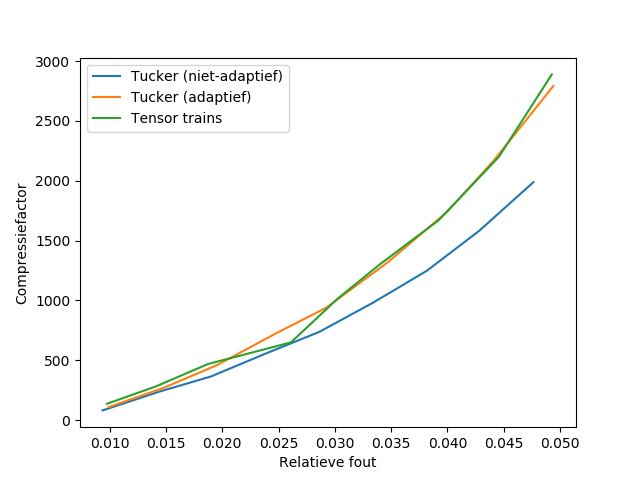
\includegraphics[scale=0.5]{images/tucker_vs_tensor_trains_Cuprite.png}
\end{figure}

\end{frame}

\begin{frame}{Tucker vs tensor trains: Mauna Kea}

\begin{figure}[H]
\centering
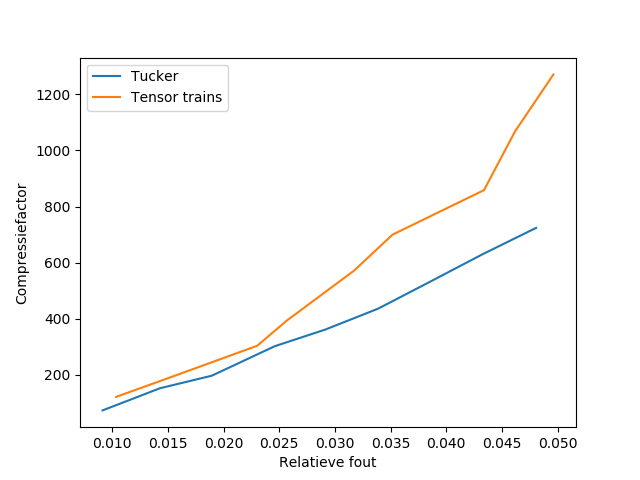
\includegraphics[scale=0.5]{images/tucker_vs_tensor_trains_Mauna_Kea.png}
\end{figure}

\end{frame}

\begin{frame}{Compressietijd: Cuprite}

\begin{figure}[H]
\centering
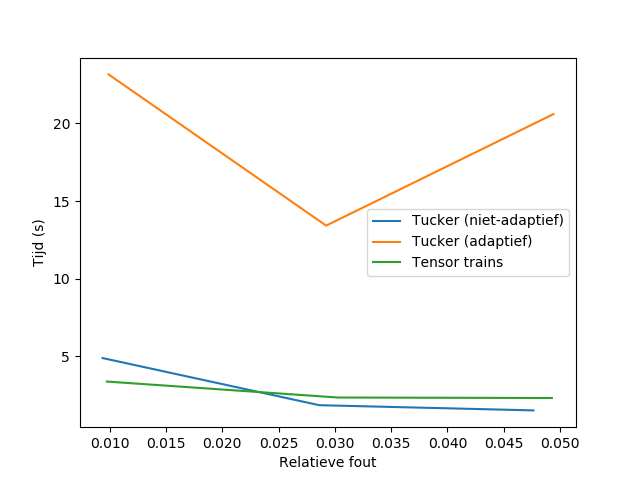
\includegraphics[scale=0.5]{images/tucker_vs_tensor_trains_times_Cuprite.png}
\end{figure}

\end{frame}

\begin{frame}{Compressietijd: Mauna Kea}

\begin{figure}[H]
\centering
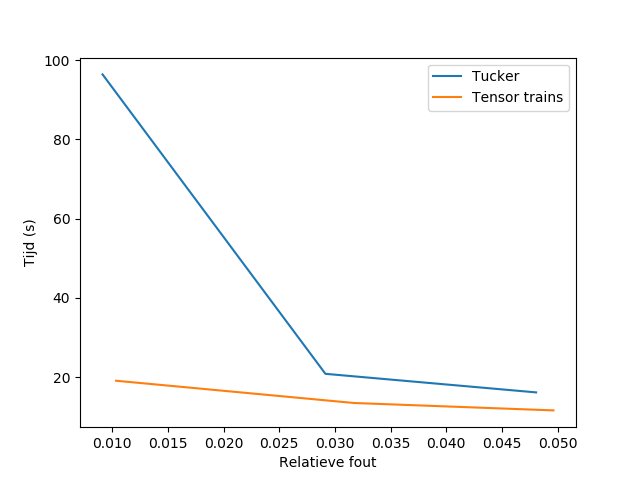
\includegraphics[scale=0.5]{images/tucker_vs_tensor_trains_times_Mauna_Kea.png}
\end{figure}

\end{frame}

\begin{frame}{Algemene \textit{lossy} compressie}

\begin{itemize}
\item JPEG: bundel elke 3 opeenvolgende spectrale banden als JPEG-afbeelding
\item x264:
\begin{itemize}
\item Videocompressor
\item Beschouw 3D-tensor als video met 1 frame/spectrale band
\item Preset (bv. medium of ultrafast) bepaalt compressietijd
\end{itemize}
\end{itemize}

\end{frame}

\begin{frame}{Algemene vergelijking: Cuprite}

\begin{figure}[H]
\centering
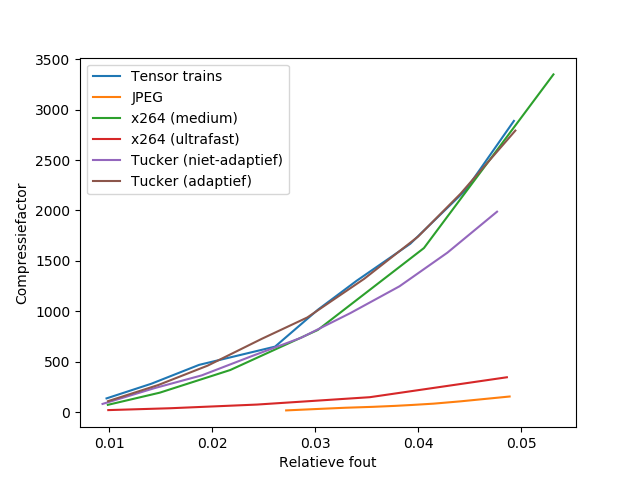
\includegraphics[scale=0.5]{images/general_comparison_new_Cuprite.png}
\end{figure}

\end{frame}

\begin{frame}{Algemene vergelijking: Mauna Kea}

\begin{figure}[H]
\centering
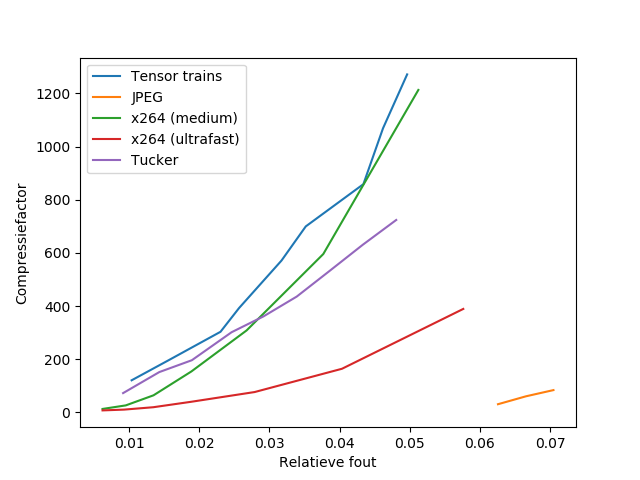
\includegraphics[scale=0.5]{images/general_comparison_new_Mauna_Kea.png}
\end{figure}

\end{frame}

\begin{frame}{Compressietijd: Cuprite}

\begin{figure}[H]
\centering
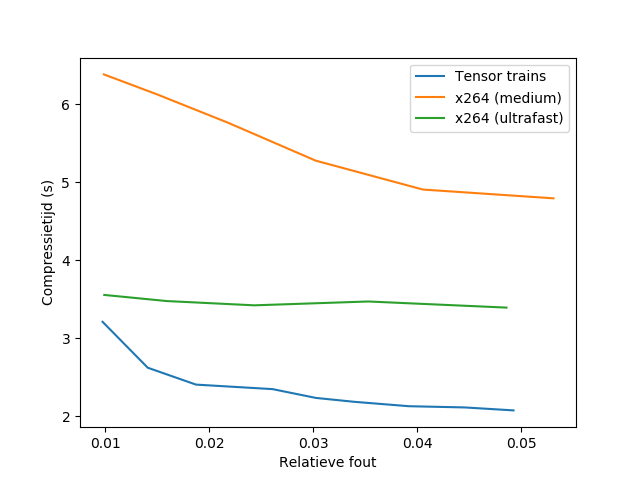
\includegraphics[scale=0.5]{images/general_comparison_times_Cuprite.png}
\end{figure}

\end{frame}

\begin{frame}{Compressietijd: Mauna Kea}

\begin{figure}[H]
\centering
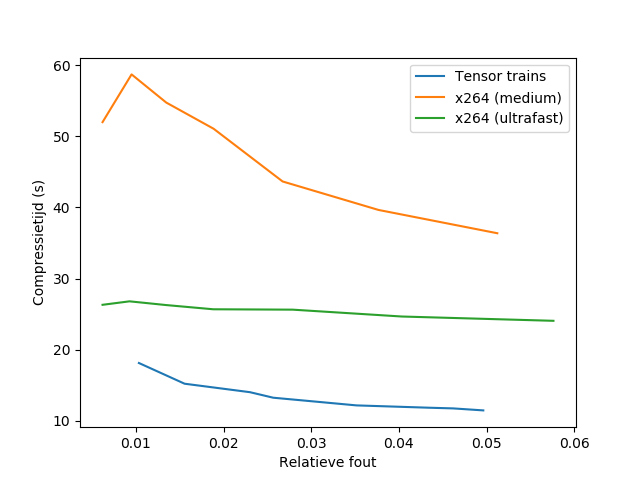
\includegraphics[scale=0.5]{images/general_comparison_times_Mauna_Kea.png}
\end{figure}

\end{frame}

\begin{frame}{Compressietijd: Pavia Centre}

\begin{figure}[H]
\centering
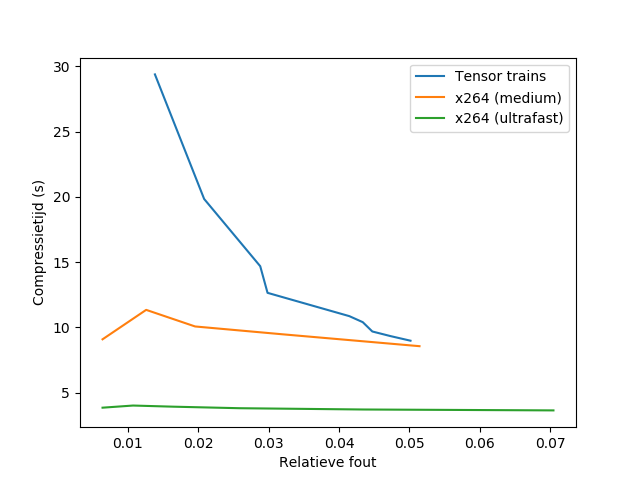
\includegraphics[scale=0.5]{images/general_comparison_times_Pavia_Centre.png}
\end{figure}

\end{frame}

\begin{frame}{Voorbeeldcompressies}

\begin{table}[H]
\centering
\begin{tabular}{C{0.6\textwidth}  L{0.4\textwidth}}
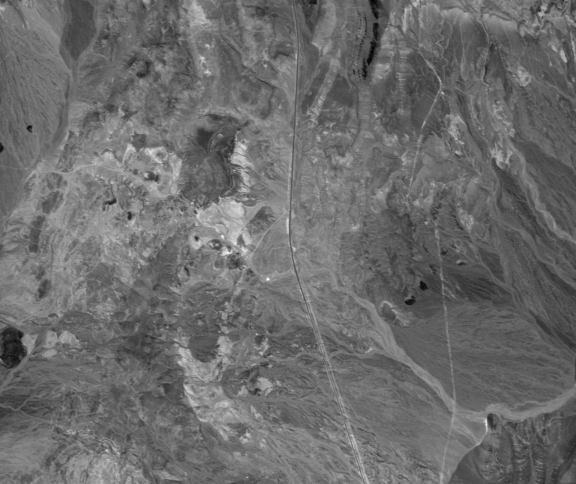
\includegraphics[width=\linewidth]{images/cuprite_cropped_sum.png}
&
Cuprite (VS)\newline
Bron: AVIRIS \cite{ref:ehu_aviris_cuprite}\newline
\vspace{5mm}
Relatieve fout: 0
Compressiefactor: 1
\end{tabular}
\end{table}

\end{frame}

\begin{frame}{Voorbeeldcompressies}

\begin{table}[H]
\centering
\begin{tabular}{C{0.6\textwidth}  L{0.4\textwidth}}
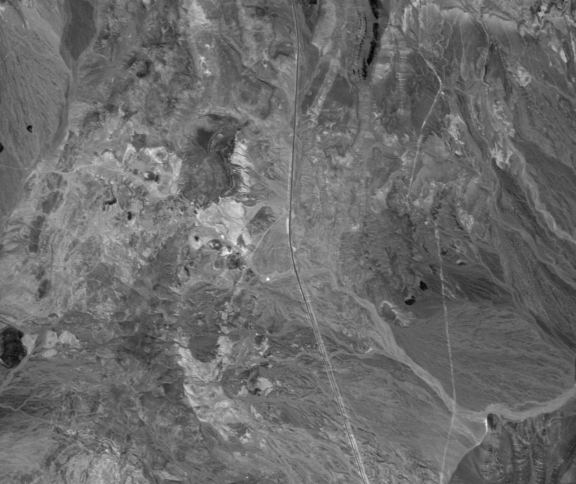
\includegraphics[width=\linewidth]{images/example_compression_Cuprite_0_01.png}
&
Cuprite (VS)\newline
Bron: AVIRIS \cite{ref:ehu_aviris_cuprite}\newline
\vspace{5mm}
Relatieve fout: 0.0098
Compressiefactor: 136.2
\end{tabular}
\end{table}

\end{frame}

\begin{frame}{Voorbeeldcompressies}

\begin{table}[H]
\centering
\begin{tabular}{C{0.6\textwidth}  L{0.4\textwidth}}
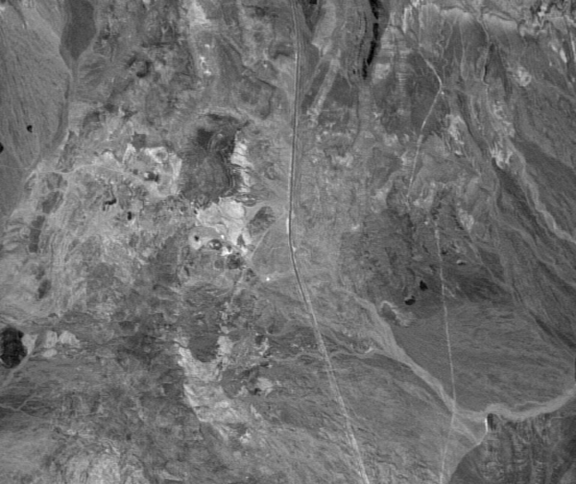
\includegraphics[width=\linewidth]{images/example_compression_Cuprite_0_025.png}
&
Cuprite (VS)\newline
Bron: AVIRIS \cite{ref:ehu_aviris_cuprite}\newline
\vspace{5mm}
Relatieve fout: 0.0261
Compressiefactor: 649.6
\end{tabular}
\end{table}

\end{frame}

\begin{frame}{Voorbeeldcompressies}

\begin{table}[H]
\centering
\begin{tabular}{C{0.6\textwidth}  L{0.4\textwidth}}
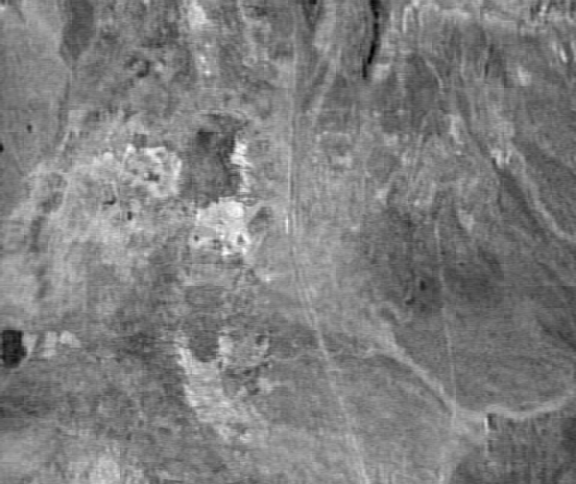
\includegraphics[width=\linewidth]{images/example_compression_Cuprite_0_05.png}
&
Cuprite (VS)\newline
Bron: AVIRIS \cite{ref:ehu_aviris_cuprite}\newline
\vspace{5mm}
Relatieve fout: 0.0493
Compressiefactor: 2888.5
\end{tabular}
\end{table}

\end{frame}

\begin{frame}{Voorbeeldcompressies}

\begin{table}[H]
\centering
\begin{tabular}{C{0.6\textwidth}  L{0.4\textwidth}}
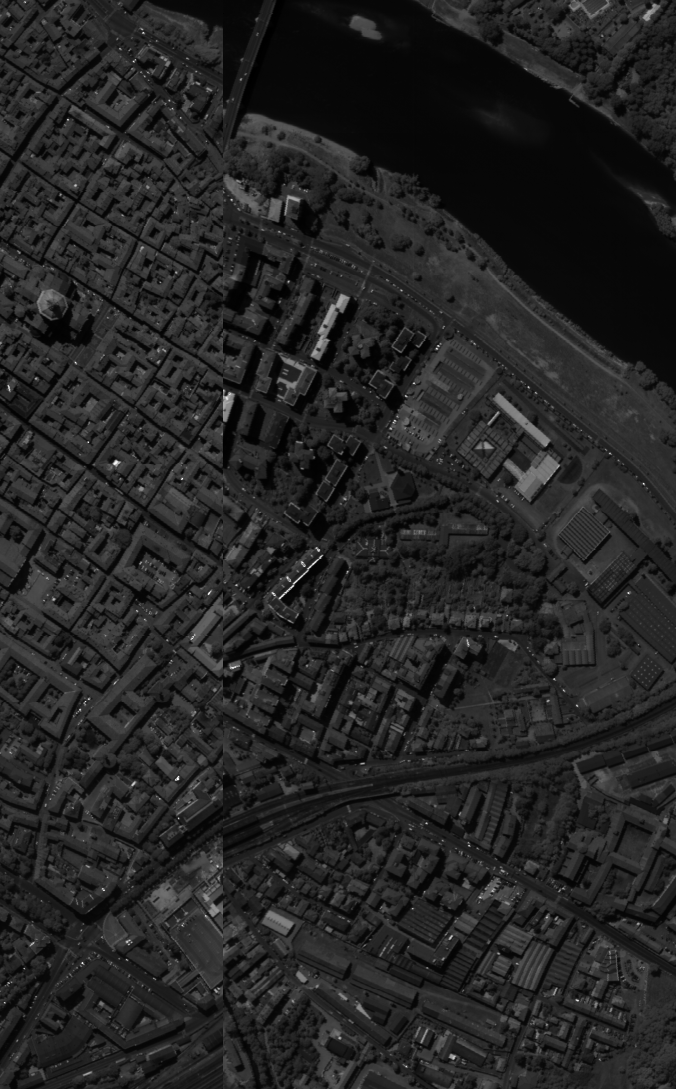
\includegraphics[height=6cm]{images/pavia_sum.png}
&
Pavia Centre (Itali\"e)\newline
Bron: ROSIS \cite{ref:ehu_rosis_pavia_centre}\newline
\vspace{5mm}
Relatieve fout: 0
Compressiefactor: 1
\end{tabular}
\end{table}

\end{frame}

\begin{frame}{Voorbeeldcompressies}

\begin{table}[H]
\centering
\begin{tabular}{C{0.6\textwidth}  L{0.4\textwidth}}
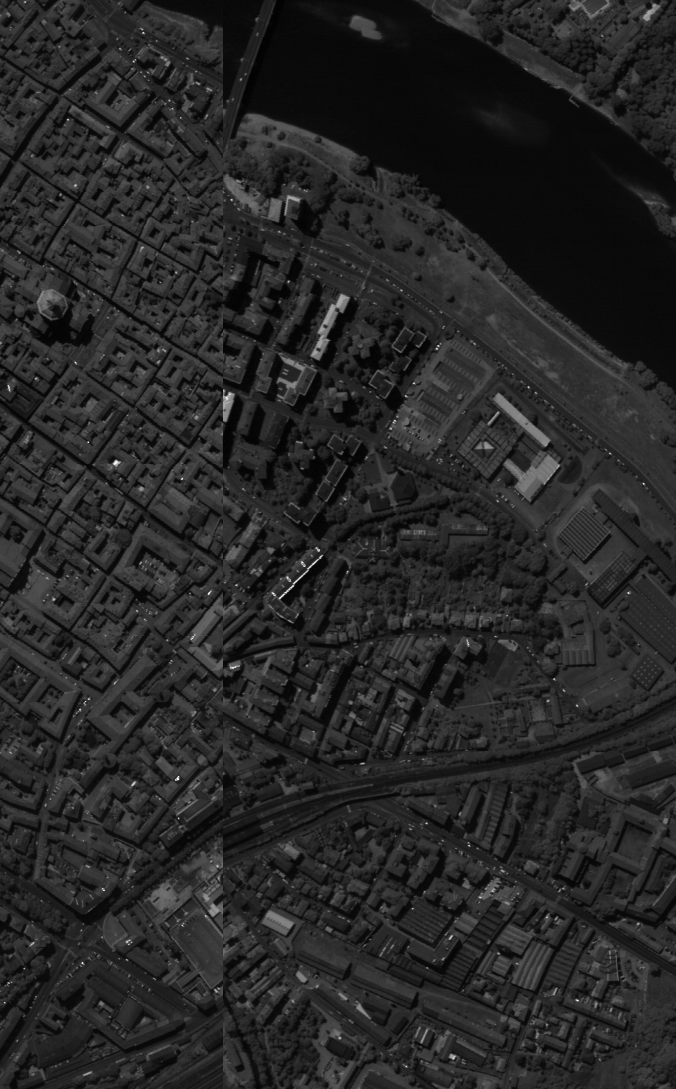
\includegraphics[height=6cm]{images/example_compression_Pavia_Centre_0_05.png}
&
Pavia Centre (Itali\"e)\newline
Bron: ROSIS \cite{ref:ehu_rosis_pavia_centre}\newline
\vspace{5mm}
Relatieve fout: 0.0502
Compressiefactor: 90.7
\end{tabular}
\end{table}

\end{frame}

\begin{frame}{Voorbeeldcompressies}

\begin{table}[H]
\centering
\begin{tabular}{C{0.6\textwidth}  L{0.4\textwidth}}
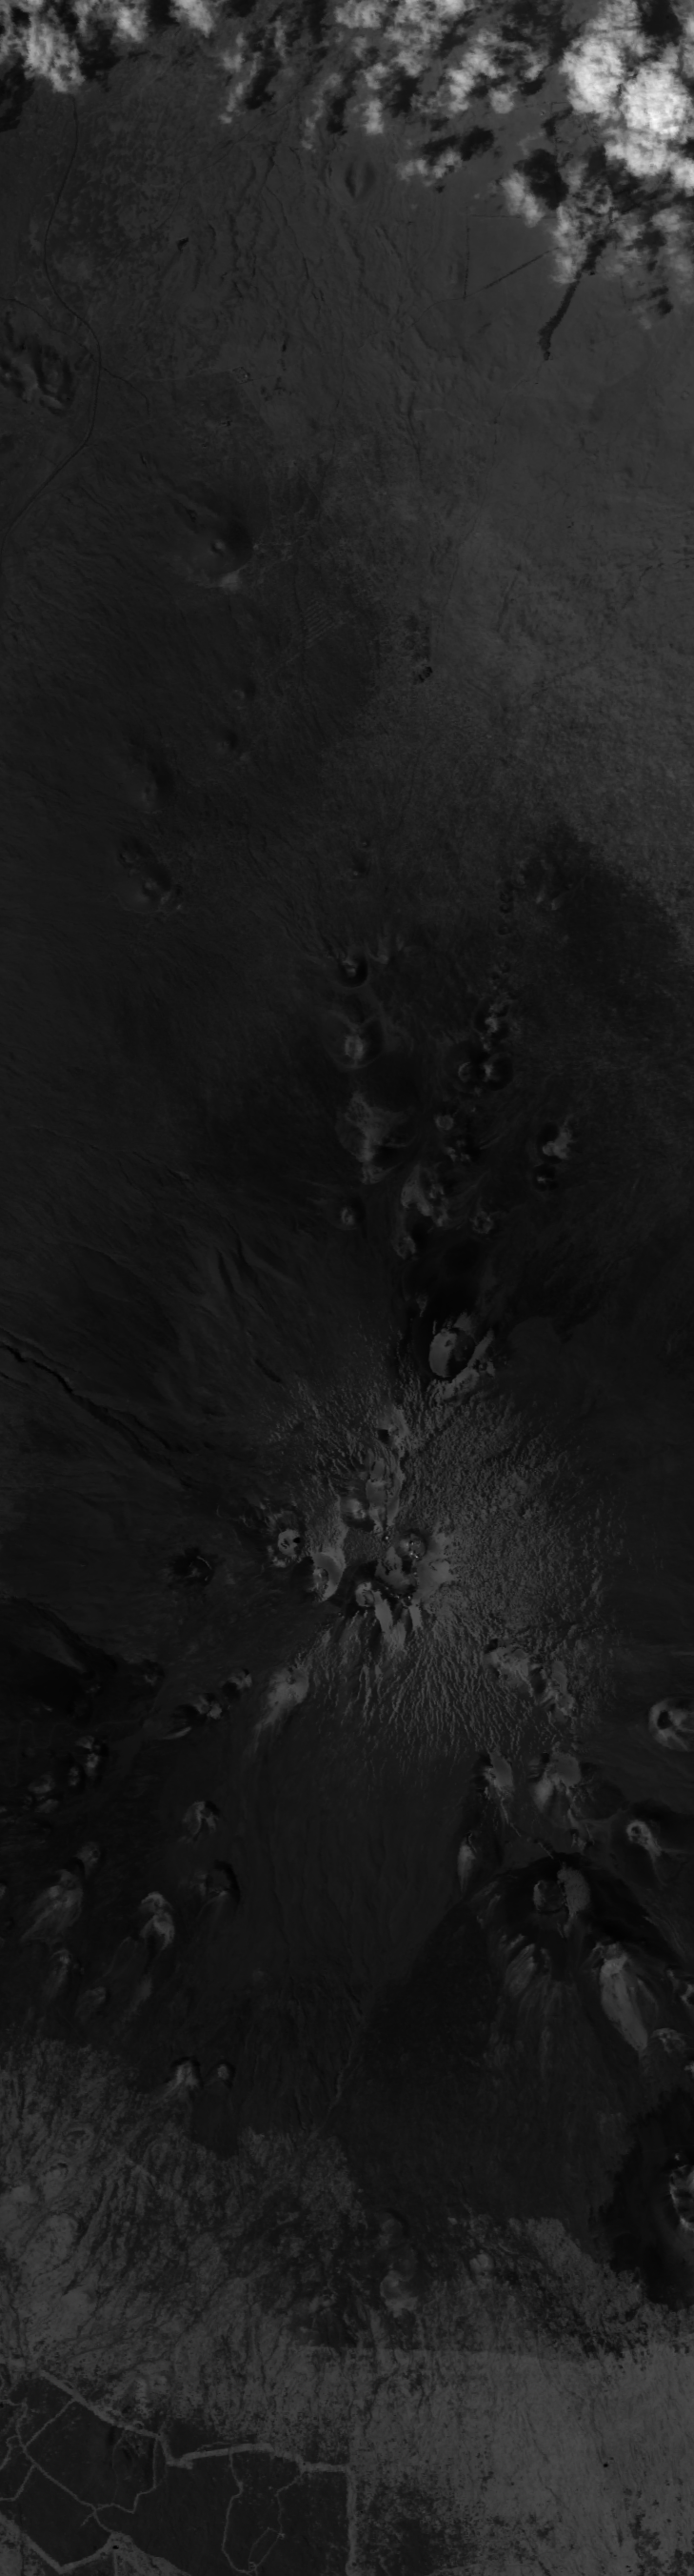
\includegraphics[height=6cm]{images/mauna_kea_sum.png}
&
Mauna Kea (VS)\newline
Bron: AVIRIS \cite{ref:aviris}\newline
\vspace{5mm}
Relatieve fout: 0
Compressiefactor: 1
\end{tabular}
\end{table}

\end{frame}

\begin{frame}{Voorbeeldcompressies}

\begin{table}[H]
\centering
\begin{tabular}{C{0.6\textwidth}  L{0.4\textwidth}}
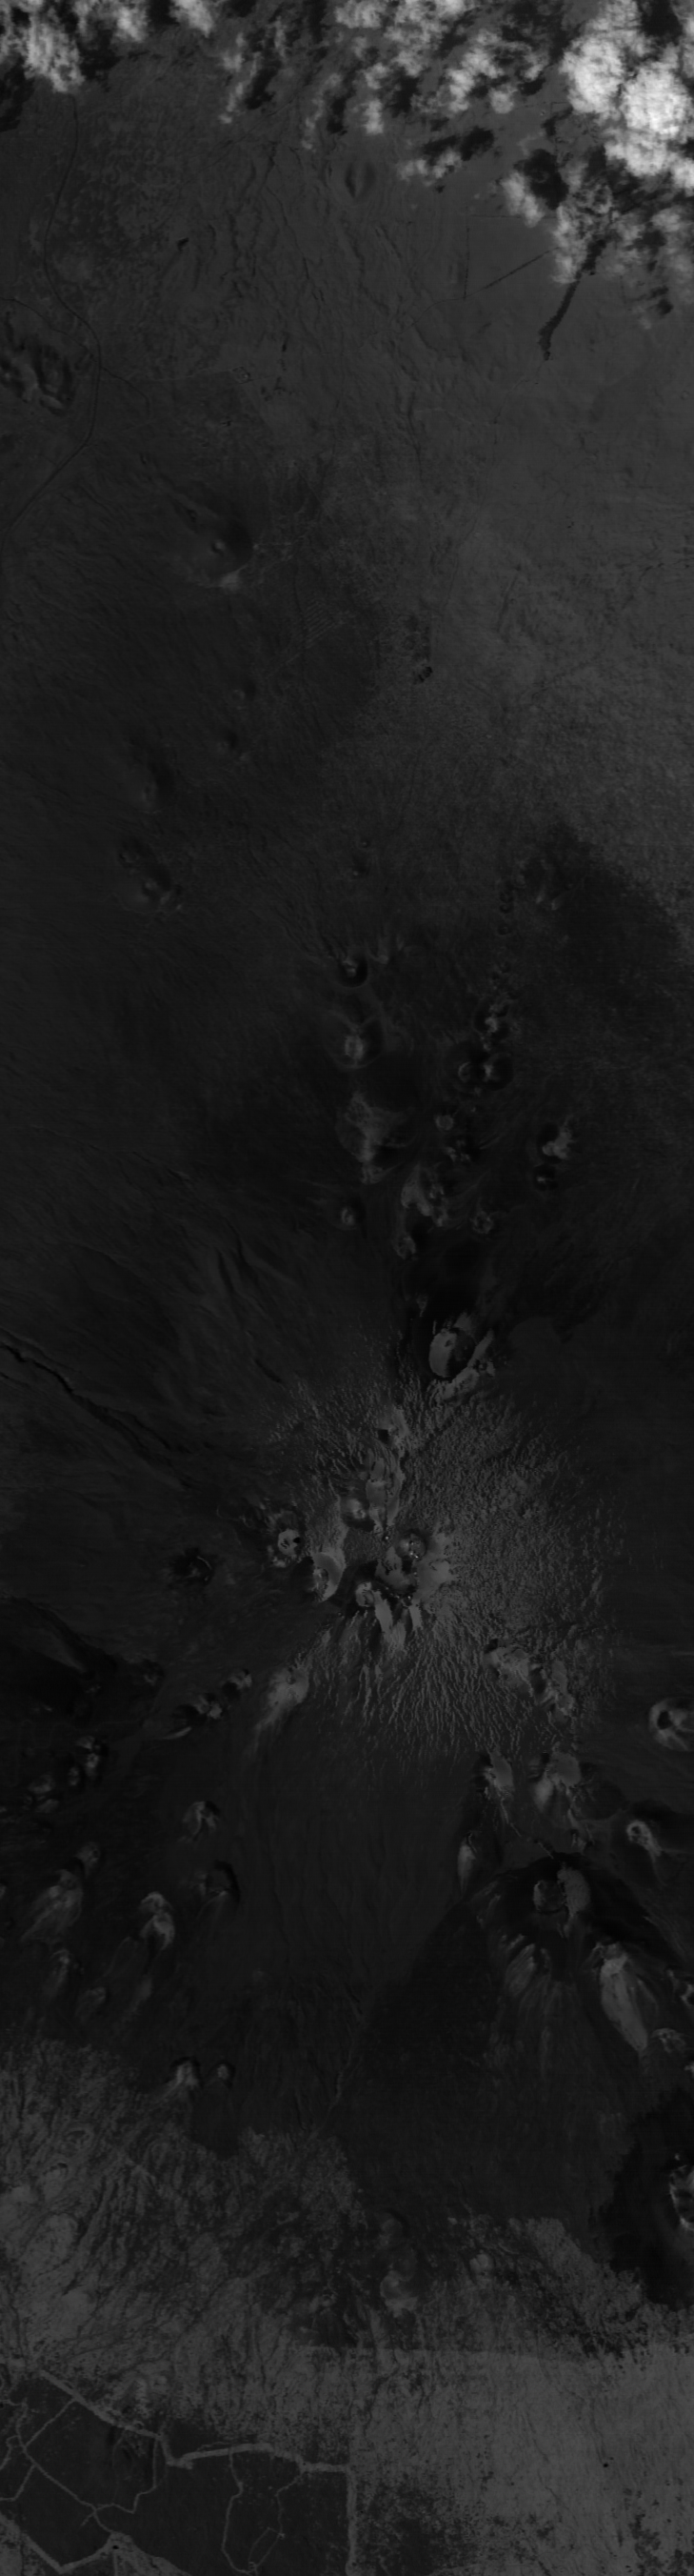
\includegraphics[height=6cm]{images/example_compression_Mauna_Kea_0_025.png}
&
Mauna Kea (VS)\newline
Bron: AVIRIS \cite{ref:aviris}\newline
\vspace{5mm}
Relatieve fout: 0.0257
Compressiefactor: 392.67
\end{tabular}
\end{table}

\end{frame}

\begin{frame}{Voorbeeldcompressies}

\begin{table}[H]
\centering
\begin{tabular}{C{0.6\textwidth}  L{0.4\textwidth}}
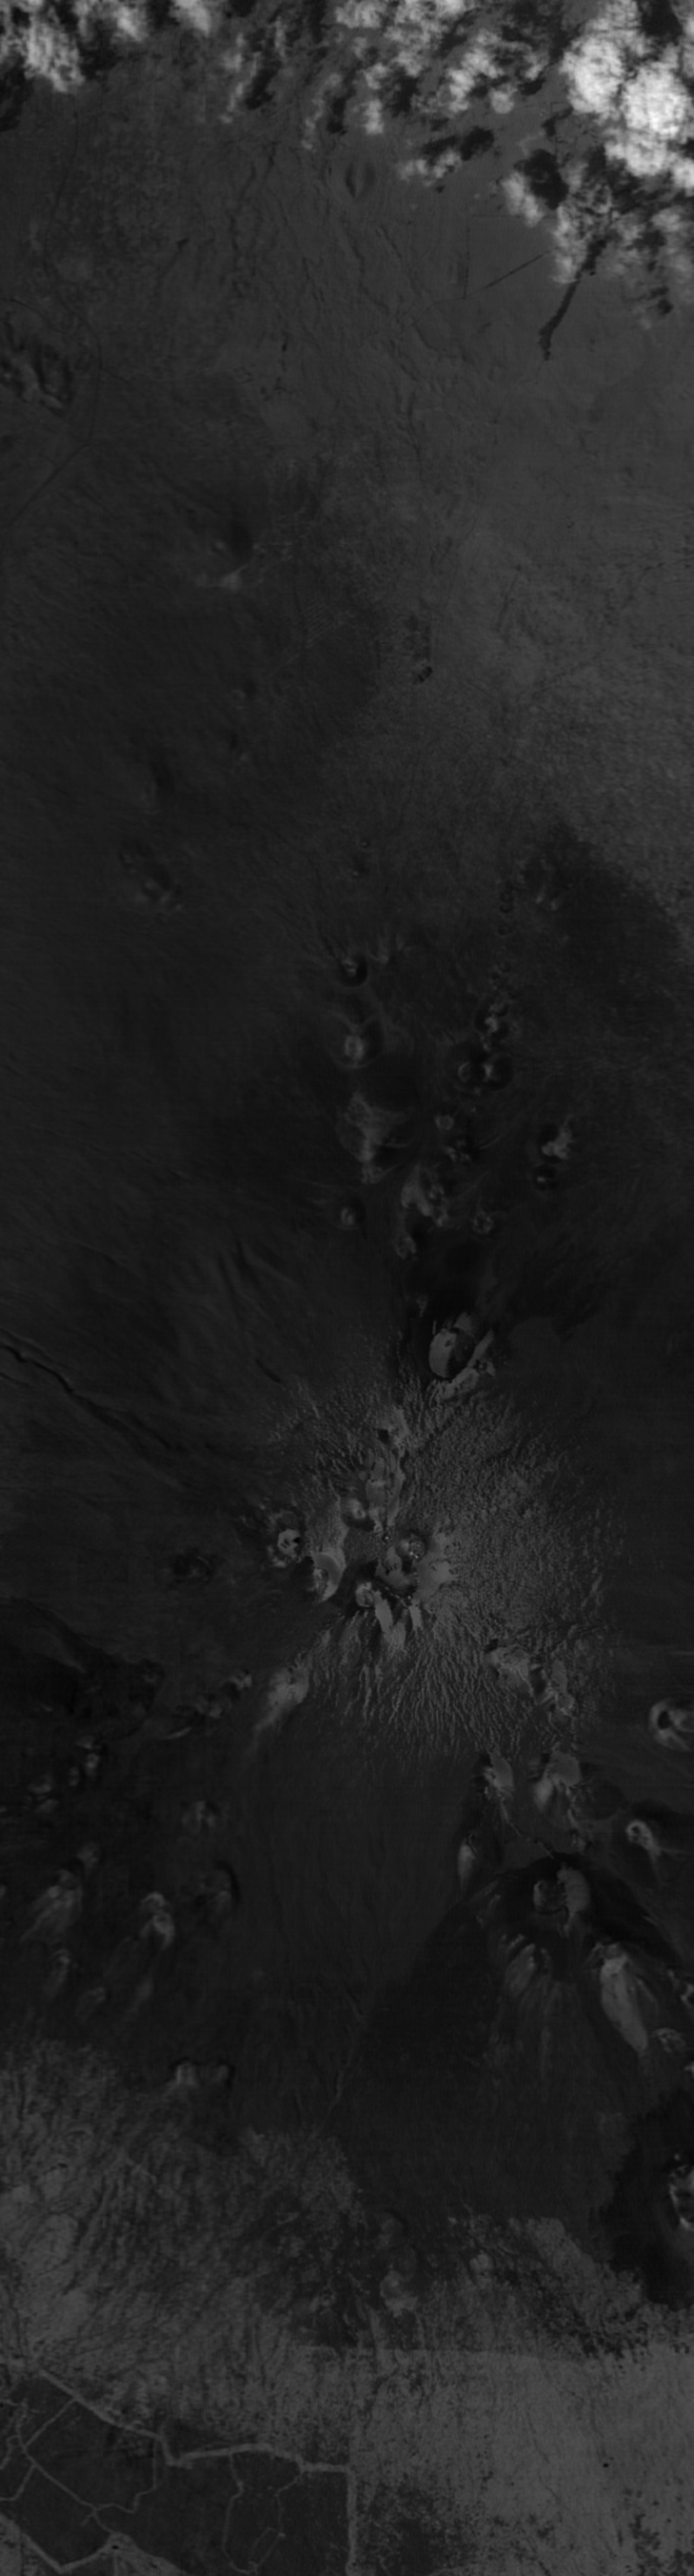
\includegraphics[height=6cm]{images/example_compression_Mauna_Kea_0_05.png}
&
Mauna Kea (VS)\newline
Bron: AVIRIS \cite{ref:aviris}\newline
\vspace{5mm}
Relatieve fout: 0.0496
Compressiefactor: 1271.31
\end{tabular}
\end{table}

\end{frame}

\begin{frame}{Verder onderzoek}
Belangrijkste pistes:
\begin{itemize}
\item Verbeterde quantisatie en encodering
\item Verbeterde parameterselectie
\item Laag-niveau implementatie
\item Combinatie met DCT
\end{itemize}
\end{frame}

\begin{frame}{Referenties}
	\scriptsize
	\bibliographystyle{ieeetr}
	\bibliography{references.bib}
	\normalsize
\end{frame}

\end{document}
